\section*{Conclusions}

\begin{frame}{Conclusions and Future Works}

    In the work we have:
    \begin{itemize}
        \item Investigated two new dynamic problems using graph-based knowledge;
        \item proposed algorithms efficiently solving the problem variants;
        \item the algorithms (\DPASATAlgorithmName{}, \DOHSATAlgorithmName{}, \CPDSearch{}) have been experimentally evaluated. The analysis shows significant gains \wrt{} \stateofart{};

        \item \textbf{Future works}: 
            The decremental consistency checking problem can be investigated in other algebra (\eg{} spatial); 
            or it can be use to find the minimal set of constraint relaxation making an inconsistent \TCSPName{} consistent;
            \CPDSearch{} can be (possibly) further improved by integrating a focal list to improve performance (\eg{} when the early termination mechanism is of little help).
    \end{itemize}
\end{frame}

\usebackgroundtemplate{%
	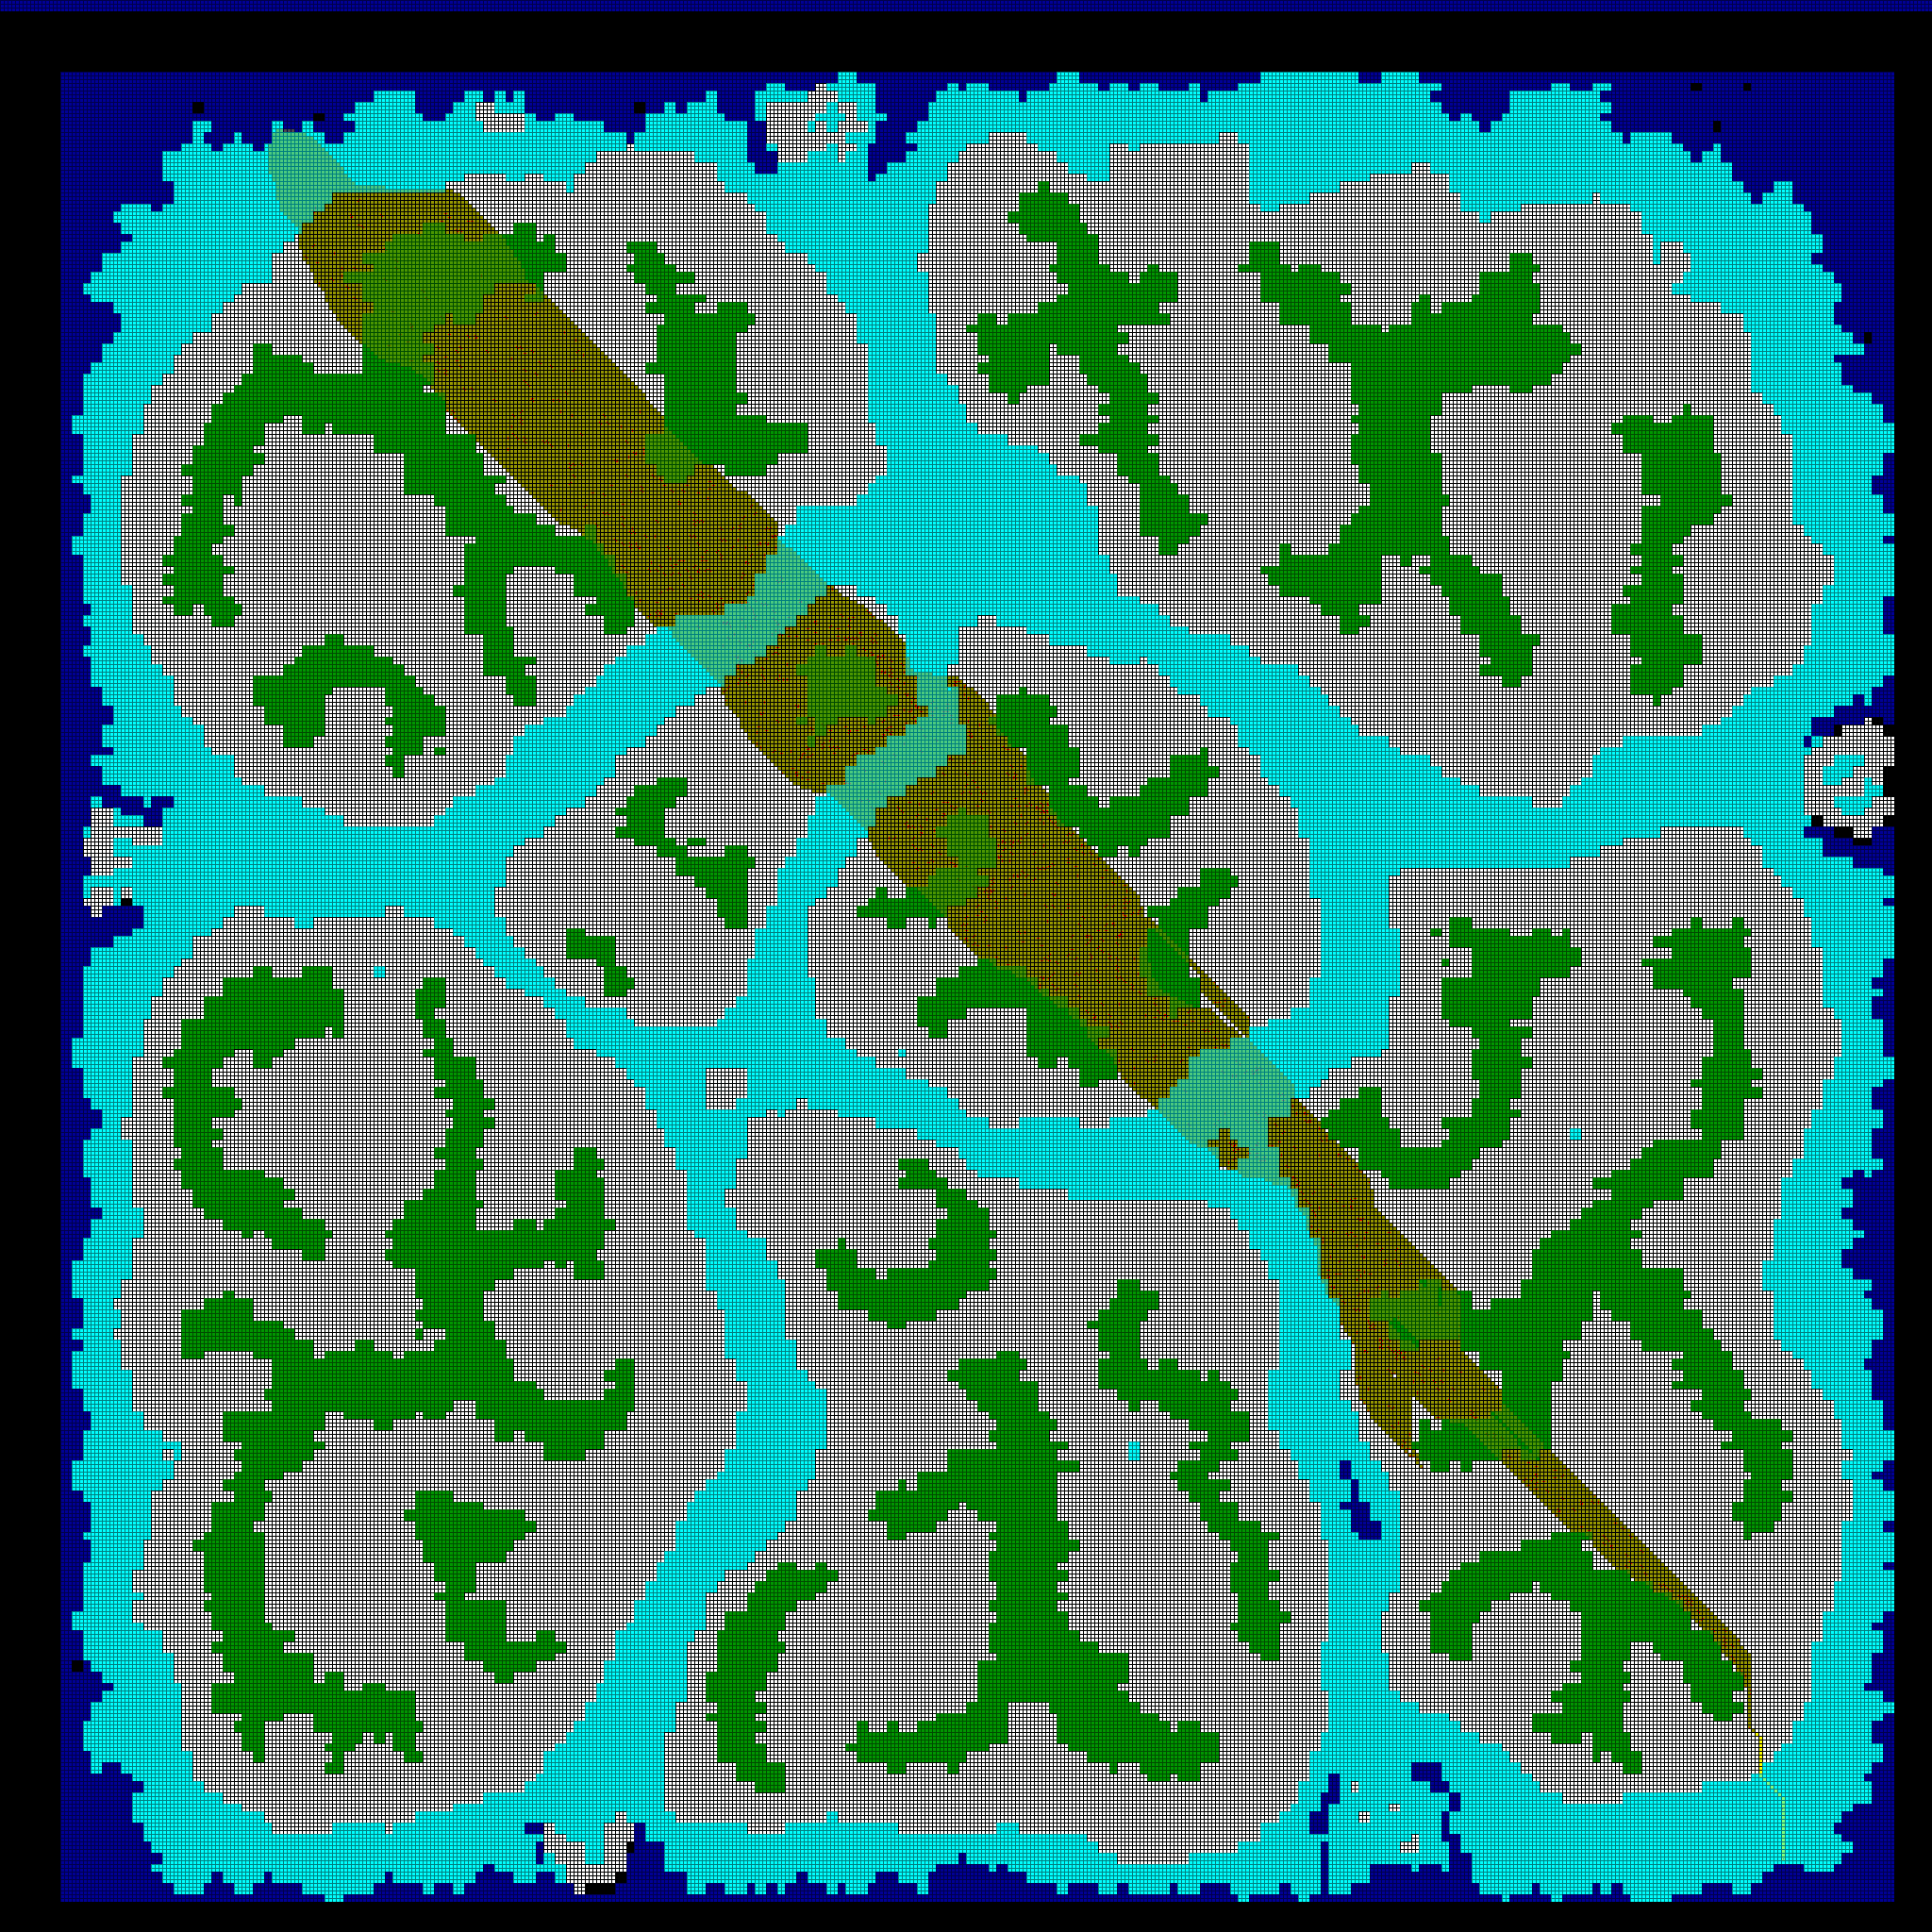
\includegraphics[width=\paperwidth,height=\paperheight]{src/images/pathfinding/cpdsearch}%
}
\begin{frame}[plain]
    \centering \Huge \textbf{Thanks for listening!\\Questions???}
\end{frame}
